%% LyX 1.4.3 created this file.  For more info, see http://www.lyx.org/.
%% Do not edit unless you really know what you are doing.
\documentclass[english]{amsbook}
\usepackage[T1]{fontenc}
\usepackage[latin1]{inputenc}
\usepackage{geometry}
\geometry{verbose,letterpaper,tmargin=1in,bmargin=1in,lmargin=1.3in,rmargin=1.3in}
\pagestyle{headings}
\usepackage{graphicx}
\usepackage{amssymb}
\IfFileExists{url.sty}{\usepackage{url}}
                      {\newcommand{\url}{\texttt}}

\makeatletter
%%%%%%%%%%%%%%%%%%%%%%%%%%%%%% Textclass specific LaTeX commands.
 \theoremstyle{plain}
\newtheorem{thm}{Theorem}[section]

%%%%%%%%%%%%%%%%%%%%%%%%%%%%%% User specified LaTeX commands.
% Common preamble for all included files.  If writing them in LyX, simply set
% in the preamble the line:
% % Common preamble for all included files.  If writing them in LyX, simply set
% in the preamble the line:
% % Common preamble for all included files.  If writing them in LyX, simply set
% in the preamble the line:
% \input{preamble.tex}
% This will allow you to compile/view any individual file without having to
% recompile starting from the entire master.

% This gives us a better font in URL links (otherwise the default 
% MonoSpace font is bitmapped, and it looks horrible in PDF)
\usepackage{courier}

% Special-purpose color definitions
\usepackage{color}
\definecolor{orange}{cmyk}{0,0.4,0.8,0.2}

% The hyperref package gives us a pdf with properly built 
% internal navigation ('pdf bookmarks' for the table of contents,
% internal cross-reference links, web links for URLs, etc.)

% A few colors to replace the defaults for certain link types
\definecolor{darkorange}{rgb}{.71,0.21,0.01}
\definecolor{darkgreen}{rgb}{.12,.54,.11}

\usepackage[pdftex,  % needed for pdflatex
  breaklinks=true,  % so long urls are correctly broken across lines
  colorlinks=true,
  urlcolor=blue,
  linkcolor=darkorange,
  citecolor=darkgreen,
  ]{hyperref}

% This helps prevent overly long lines that stretch beyond the margins
\sloppy

% Use and configure listings package for nicely formatted code
\usepackage{listings}
\lstset{
  language=Python,
  basicstyle=\small\ttfamily,
  commentstyle=\ttfamily\color{blue},
  stringstyle=\ttfamily\color{darkorange},
  showstringspaces=false,
  breaklines=true,
  postbreak = \space\dots
}

% Some extra commands

\newcommand{\fig}[4]
{\begin{figure}[ht]
\begin{center}
\includegraphics[width=#1]{#2}
\caption{\label{#4} #3}
\end{center}
\end{figure}}

\newcommand{\matlab}[0]{matlab{\texttrademark}}
\newcommand{\fname}[1]{{\tt #1}}
\newcommand{\func}[1]{{\tt #1}}
\newcommand{\class}[1]{{\tt #1}}
\newcommand{\mpldoc}[1]{{\tt #1}}

\newcommand{\code}[1]{{\tt #1}}
\newcommand{\prompt}[1]{\code{>>> #1}}
\newcommand{\carg}[1]{\textit{#1}} % command argument
\newcommand{\val}[1]{\textit{#1}}
\newcommand{\rc}[1]{{\tt #1}}

% no-op for a sequence that was created when importing the
% mayavi chapter.  This prevents latex errors.
\newcommand{\dbz}{ }

% This will allow you to compile/view any individual file without having to
% recompile starting from the entire master.

% This gives us a better font in URL links (otherwise the default 
% MonoSpace font is bitmapped, and it looks horrible in PDF)
\usepackage{courier}

% Special-purpose color definitions
\usepackage{color}
\definecolor{orange}{cmyk}{0,0.4,0.8,0.2}

% The hyperref package gives us a pdf with properly built 
% internal navigation ('pdf bookmarks' for the table of contents,
% internal cross-reference links, web links for URLs, etc.)

% A few colors to replace the defaults for certain link types
\definecolor{darkorange}{rgb}{.71,0.21,0.01}
\definecolor{darkgreen}{rgb}{.12,.54,.11}

\usepackage[pdftex,  % needed for pdflatex
  breaklinks=true,  % so long urls are correctly broken across lines
  colorlinks=true,
  urlcolor=blue,
  linkcolor=darkorange,
  citecolor=darkgreen,
  ]{hyperref}

% This helps prevent overly long lines that stretch beyond the margins
\sloppy

% Use and configure listings package for nicely formatted code
\usepackage{listings}
\lstset{
  language=Python,
  basicstyle=\small\ttfamily,
  commentstyle=\ttfamily\color{blue},
  stringstyle=\ttfamily\color{darkorange},
  showstringspaces=false,
  breaklines=true,
  postbreak = \space\dots
}

% Some extra commands

\newcommand{\fig}[4]
{\begin{figure}[ht]
\begin{center}
\includegraphics[width=#1]{#2}
\caption{\label{#4} #3}
\end{center}
\end{figure}}

\newcommand{\matlab}[0]{matlab{\texttrademark}}
\newcommand{\fname}[1]{{\tt #1}}
\newcommand{\func}[1]{{\tt #1}}
\newcommand{\class}[1]{{\tt #1}}
\newcommand{\mpldoc}[1]{{\tt #1}}

\newcommand{\code}[1]{{\tt #1}}
\newcommand{\prompt}[1]{\code{>>> #1}}
\newcommand{\carg}[1]{\textit{#1}} % command argument
\newcommand{\val}[1]{\textit{#1}}
\newcommand{\rc}[1]{{\tt #1}}

% no-op for a sequence that was created when importing the
% mayavi chapter.  This prevents latex errors.
\newcommand{\dbz}{ }

% This will allow you to compile/view any individual file without having to
% recompile starting from the entire master.

% This gives us a better font in URL links (otherwise the default 
% MonoSpace font is bitmapped, and it looks horrible in PDF)
\usepackage{courier}

% Special-purpose color definitions
\usepackage{color}
\definecolor{orange}{cmyk}{0,0.4,0.8,0.2}

% The hyperref package gives us a pdf with properly built 
% internal navigation ('pdf bookmarks' for the table of contents,
% internal cross-reference links, web links for URLs, etc.)

% A few colors to replace the defaults for certain link types
\definecolor{darkorange}{rgb}{.71,0.21,0.01}
\definecolor{darkgreen}{rgb}{.12,.54,.11}

\usepackage[pdftex,  % needed for pdflatex
  breaklinks=true,  % so long urls are correctly broken across lines
  colorlinks=true,
  urlcolor=blue,
  linkcolor=darkorange,
  citecolor=darkgreen,
  ]{hyperref}

% This helps prevent overly long lines that stretch beyond the margins
\sloppy

% Use and configure listings package for nicely formatted code
\usepackage{listings}
\lstset{
  language=Python,
  basicstyle=\small\ttfamily,
  commentstyle=\ttfamily\color{blue},
  stringstyle=\ttfamily\color{darkorange},
  showstringspaces=false,
  breaklines=true,
  postbreak = \space\dots
}

% Some extra commands

\newcommand{\fig}[4]
{\begin{figure}[ht]
\begin{center}
\includegraphics[width=#1]{#2}
\caption{\label{#4} #3}
\end{center}
\end{figure}}

\newcommand{\matlab}[0]{matlab{\texttrademark}}
\newcommand{\fname}[1]{{\tt #1}}
\newcommand{\func}[1]{{\tt #1}}
\newcommand{\class}[1]{{\tt #1}}
\newcommand{\mpldoc}[1]{{\tt #1}}

\newcommand{\code}[1]{{\tt #1}}
\newcommand{\prompt}[1]{\code{>>> #1}}
\newcommand{\carg}[1]{\textit{#1}} % command argument
\newcommand{\val}[1]{\textit{#1}}
\newcommand{\rc}[1]{{\tt #1}}

% no-op for a sequence that was created when importing the
% mayavi chapter.  This prevents latex errors.
\newcommand{\dbz}{ }


\usepackage{babel}
\makeatother
\begin{document}

\title{ \vspace{3cm} Practical Scientific Computing\\
in Python\\
A Workbook}


\author{ \vspace{1cm} John D. Hunter\\
Fernando P�rez \vspace{1cm} }

\maketitle
\tableofcontents{}


\chapter{Introduction}

This document contains a set of small problems, drawn from many different
fields, meant to illustrate commonly useful techniques for using Python
in scientific computing.

All problems are presented in a similar fashion: the task is explained
including any necessary mathematical background and a `code skeleton'
is provided that is meant to serve as a starting point for the solution
of the exercise. In some cases, some example output of the expected
solution, figures or additional hints may be provided as well. 

The accompanying source download for this workbook contains the complete
solutions, which are not part of this document for the sake of brevity.

For several examples, the provided skeleton contains pre-written tests
which validate the correctness of the expected answers. When you have
completed the exercise successfully, you should be able to run it
from within IPython and see something like this (illustrated using
a trapezoidal rule problem, whose solution is in the file \texttt{trapezoid.py}):

\begin{lstlisting}
In [7]: run trapezoid.py
....
----------------------------------------------------------------------
Ran 4 tests in 0.003s

OK
\end{lstlisting}

This message tells you that 4 automatic tests were successfully executed.
The idea of including automatic tests in your code is a common one
in modern software development, and Python includes in its standard
library two modules for automatic testing, with slightly different
functionality: \texttt{unittest} and \texttt{doctest}. These tests
were written using the \texttt{unittest} system, whose complete documentation
can be found here: \url{http://docs.python.org/lib/module-unittest.html}. 

Other exercises will illustrate the use of the \texttt{doctest} system,
since it provides complementary functionality.



\chapter{Simple non-numerical problems}

\section{Sorting quickly with QuickSort }

\textbf{Illustrates}: lists, recursion.

Quicksort is one of the best known, and probably the simplest, fast
algorithm for sorting $n$ items. It is fast in the sense that it
requires on average $\mathcal{O}(n\log n)$ comparisons instead of
$\mathcal{O}(n^{2})$, although a naive implementation does have quadratic
worst-case behavior.

The algorithm uses a simple divide and conquer strategy, and its implementation
is naturally recursive. Its basic steps are:

\begin{enumerate}
\item Pick an element from the list, called the pivot $p$ (any choice works).
\item Select from the rest of the list those elements smaller and those
greater than the pivot, and store them in separate lists $S$ and
$G$.
\item Recursively apply the algorithm \texttt{}to $S$ and $G$. The final
result can be written as $\sigma(S)+[p]+\sigma(G)$, where $\sigma$
represents the sorting operation, $+$ indicates list concatenation
and $[p]$ is the list containing the pivot as its single element.
\end{enumerate}
The listing~\ref{code:qsort} contains a skeleton with no implementation
but with tests already written (in the form of \emph{unit tests},
as described in the introduction).

\lstinputlisting[label=code:qsort,caption={IGNORED}]{problems/qsort.py}


\subsection*{Hints}

\begin{itemize}

\item Python has no particular syntactic requirements for implementing
  recursion, but it does have a maximum recursion depth. This value can be
  queried via the function \texttt{sys.getrecursionlimit()}, and it can be
  changed with \texttt{sys.setrecursionlimit(new\_value)}.

\item Like in all recursive problems, don't forget to implement an exit
  condition!

\item If \texttt{L} is a list, the call \texttt{len(L)} provides its length.

\end{itemize}




\section{Dictionaries for counting words}

A common task in text processing is to produce a count of word frequencies.
While NumPy has a builtin histogram function for doing numerical histograms,
it won't work out of the box for couting discrete items, since it
is a binning histogram for a range of real values.

But the Python language provides very powerful string manipulation
capabilities, as well as a very flexible and efficiently implemented
builtin data type, the \emph{dictionary}, that makes this task a very
simple one.

In this problem, you will need to count the frequencies of all the
words contained in a compressed text file supplied as input. 

The listing~\ref{code:wordfreqs} contains a skeleton for this
problem, with \texttt{XXX} marking various places that are incomplete. 

\lstinputlisting[label=code:wordfreqs,caption={IGNORED}]{problems/wordfreqs.py}


\subsection*{Hints}

\begin{itemize}
\item The \texttt{print\_vk} function is already provided for you as a simple
way to summarize your results.
\item You will need to read the compressed file \texttt{HISTORY.gz}. Python
has facilities to do this without having to manually uncompress it.
\item Consider `words' simply the result of splitting the input text into
a list, using any form of whitespace as a separator. This is obviously
a very na�ve definition of `word', but it shall suffice for the purposes
of this exercise.
\item Python strings have a \texttt{.split()} method that allows for very
flexible splitting. You can easily get more details on it in IPython:
\end{itemize}
\begin{lstlisting}
In [2]: a = 'somestring'

In [3]: a.split?
Type:           builtin_function_or_method
Base Class:     <type 'builtin_function_or_method'>
Namespace:      Interactive
Docstring:
    S.split([sep [,maxsplit]]) -> list of strings

    Return a list of the words in the string S, using sep as the
    delimiter string.  If maxsplit is given, at most maxsplit
    splits are done. If sep is not specified or is None, any
    whitespace string is a separator.
\end{lstlisting}

The complete set of methods of Python strings can be viewed by hitting
the TAB key in IPython after typing `\texttt{a.}', and each of them
can be similarly queried with the `\texttt{?}' operator as above.
For more details on Python strings and their companion sequence types,
see
\url{http://docs.python.org/library/stdtypes.html#sequence-types-str-unicode-list-tuple-buffer-xrange}. 


\chapter{Working with files, the internet, and numpy arrays}

\section{Working with files, the web, arrays, etc\dots}
\label{sec:working_with_files}

This section is a general overview to show how easy it is to load
and manipulate data on the file system and over the web using python's
built in data structures and numpy arrays.  The goal is to exercise
basic programming skills like building filename or web addresses to
automate certain tasks like loading a series of data files or
downloading a bunch of related files off the web, as well as to
illustrate basic numpy and pylab skills.

\subsection{Loading and saving ASCII data}
\label{sec:ascii_data}

The simplest file format is a plain text ASCII file of numbers.
Although there are many better formats out there for saveing and
loading data, this format is extremely common because it has the
advantages of being human readable, and thus will survive the test of
time as the \textit{en vogue} programming languages, analysis
applications and data formats come and go, it is easy to parse, and it
is supported by almost all languages and applications.  

In this exercise we will create a data set of two arrays, the first
one regularly sampled time \textit{t} from 0..2 seconds with 20~ms
time step , and the second one an array \texttt{v} of sinusoidal
voltages corrupted by some noise.  Let's assume the sine wave has
amplitude 2~V, frequency 10~Hz, and zero mean Gaussian distrubuted
white noise with standard deviation 0.5~V.  Your task is to write two
scripts.

The first script should create the vectors \texttt{t} and \texttt{v},
plot the time series of \texttt{t} versus \texttt{v}, save them in a
two dimensional numpy array \texttt{X}, and then dump the array
\texttt{X} to a plain text ASCII file called
\texttt{'noisy_sine.dat'}.  The file will look like (not identical
because of the noise)

\begin{verbatim}
0.000000000000000000e+00 1.550947826934816025e-02
2.000000000000000042e-02 2.493944587057004725e+00
4.000000000000000083e-02 9.497694074551737975e-01
5.999999999999999778e-02 -9.185779287524413750e-01
8.000000000000000167e-02 -2.811127590689064704e+00
... and so on
\end{verbatim}

Here is the exercise skeleton of the script to create and plot the
data file

\lstinputlisting[label=code:noisy_sine_skel,caption={IGNORED}]{skel/noise_sine_skel.py}

and the graph will look something like Figure~\ref{fig:noisy_sine}

\begin{center}%
\begin{figure}
\begin{centering}\includegraphics[width=4in]{fig/noise_sine}\par\end{centering}


\caption{\label{fig:noisy_sine}A 10~Hz sine wave corrupted by noise}
\end{figure}
\par\end{center}

The second part of this exercise is to write a script which loads data
from the data file into an array \texttt{X}, extracts the columns into
arrays \texttt{t} and \texttt{v}, and computes the RMS
(root-mean-square) intensity of the signal using the \textt{load}
command.


\subsection{Loading and saving binary data}
\label{sec:binary_data}

ASCII is bloated and slow for working with large arrays, and so binary
data should be used if performance is a consideration.  To save the
array \texttt{X} in binary form, use the numpy \texttt{tostring} method

\begin{lstlisting}
# open the file for writing binary and write the binary string
file('../data/binary_data.dat', 'wb').write(X.tostring())
\end{lstlisting}

\noindent This data can later be loaded into a numpy array using
\texttt{fromstring}.  This method takes two arguments, a string and a
data type (note that numarray users can use \texttt{fromfile} which is
more efficient for importing data directly from a file).  

\lstinputlisting{code/load_binary_data.py}

\noindent Note that although Numpy and numarray use different
typecode arguments (Numeric uses strings whereas numarray uses type
objects), the matplotlib.numpy compatibility layer provides symbols
which will work with either \rc{numpy} rc setting.

\subsection{Processing several data files}
\label{sec:multiple_files}

Since python is a programming language \textit{par excellence}, it is
easy to process data in batch.  When I started the gradual transition
from a full time \matlab\ user to a full time python user, I began
processing my data in python and saving the results to data files for
plotting in \matlab.  When that became too cumbersome, I decided to
write matplotlib so I could have all the functionality I needed in one
environment.  Here is a brief example showing how to iterate over
several data files, named \fname{basename001.dat, basename002.dat,
  basename003.dat, ... basename100.dat} and plot all of the traces to
the same axes.  I'll assume for this example that each file is a 1D
ASCII array, which I can load with the \texttt{load} command.

\begin{lstlisting}
hold(True)  # set the hold state to be on
for i in range(1,101):  #start at 1, end at 100
    fname = 'basename%03d.dat'%i  # %03d pads the integers with zeros
    x = load(fname)
    plot(x)
\end{lstlisting}




\chapter{Elementary Numerics}

\section{Wallis' slow road to $\pi$}

\textbf{Illustrates}: arbitrary size integers, simple function definitions.

Wallis' formula is an infinite product that converges (slowly) to
$\pi$:\begin{equation}
\pi=\prod_{i=1}^{\infty}\frac{4i^{2}}{4i^{2}-1}.\end{equation}


The listing~\ref{code:wallis_pi} contains a skeleton with no
implementation but with some plotting commands already inserted, so
that you can visualize the convergence rate of this formula as more
terms are kept.

\lstinputlisting[label=code:wallis_pi,caption={IGNORED}]{problems/wallis_pi.py}

After running the script successfully, you should obtain a plot similar
to Figure~\ref{fig:wallis_pi}.

\begin{center}%
\begin{figure}
\begin{centering}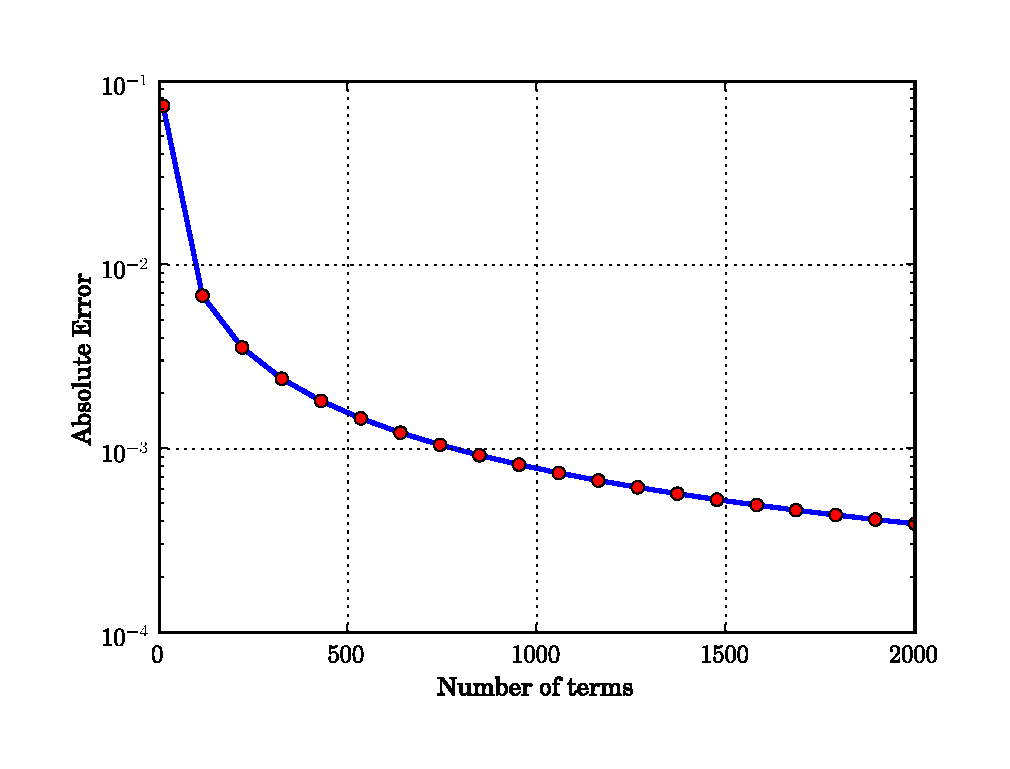
\includegraphics[width=4in]{fig/wallis_pi_convergence}\par\end{centering}


\caption{\label{fig:wallis_pi}Convergence rate for Wallis' infinite product
approximation to $\pi.$}
\end{figure}
\par\end{center}


\section{Trapezoidal rule}
\label{sec:trapezoid}

\textbf{Illustrates}: basic array slicing, functions as first class
objects.

In this exercise, you are tasked with implementing the simple trapezoid
rule formula for numerical integration. If we want to compute the
definite integral \begin{equation}
\int_{a}^{b}f(x)dx\end{equation}
we can partition the integration interval $[a,b]$ into smaller subintervals,
and approximate the area under the curve for each subinterval by the
area of the trapezoid created by linearly interpolating between the
two function values at each end of the subinterval. This is graphically
illustrated in Figure~\ref{fig:trapezoid}, where the blue line represents
the function $f(x)$ and the red line represents the successive linear
segments.

The area under $f(x)$ (the value of the definite integral) can thus
be approximated as the sum of the areas of all these trapezoids. If
we denote by $x_{i}$ ($i=0,\ldots,n,$ with $x_{0}=a$ and $x_{n}=b$)
the abscissas where the function is sampled, then \begin{equation}
\int_{a}^{b}f(x)dx\approx\frac{1}{2}\sum_{i=1}^{n}\left(x_{i}-x_{i-1}\right)\left(f(x_{i})+f(x_{i+1})\right).\label{eq:trapzf}\end{equation}
The common case of using equally spaced abscissas with spacing $h=(b-a)/n$
reads simply \begin{equation}
\int_{a}^{b}f(x)dx\approx\frac{h}{2}\sum_{i=1}^{n}\left(f(x_{i})+f(x_{i+1})\right).\label{eq:trapzf2}\end{equation}
One frequently receives the function values already precomputed, $y_{i}=f(x_{i}),$
so equation~(\ref{eq:trapzf}) becomes \begin{equation}
\int_{a}^{b}f(x)dx\approx\frac{1}{2}\sum_{i=1}^{n}\left(x_{i}-x_{i-1}\right)\left(y_{i}+y_{i-1}\right).\label{eq:trapz}\end{equation}


%
\begin{figure}
\begin{centering}\includegraphics[width=4in]{fig/Composite_trapezoidal_rule_illustration}\par\end{centering}


\caption{\label{fig:trapezoid}Illustration of the composite trapezoidal rule
with a non-uniform grid (Image credit: Wikipedia).}
\end{figure}


Listing~\ref{code:trapezoid} contains a skeleton for this problem,
written in the form of two incomplete functions and a set of automatic
tests (in the form of \emph{unit tests}, as described in the introduction).

\lstinputlisting[label=code:trapezoid,caption={IGNORED}]{problems/trapezoid.py}

In this exercise, you'll need to write two functions, \texttt{trapz}
and \texttt{trapzf}. \texttt{trapz} applies the trapezoid formula
to pre-computed values, implementing equation~(\ref{eq:trapz}),
while \texttt{trapzf} takes a function $f$ as input, as well as the
total number of samples to evaluate, and computes eq.~(\ref{eq:trapzf2}).


\section{Newton's method}
\label{sec:quad_newton}

\textbf{Illustrates:} functions as first class objects, use of the
scipy libraries.

Consider the problem of solving for $t$ in
\begin{equation}
  \int_{o}^{t}f(s)ds=u
\end{equation} 
where $f(s)$ is a monotonically increasing function of $s$ and $u>0$.

This problem can be simply solved if seen as a root finding question. Let
\begin{equation}
g(t)=\int_{o}^{t}f(s)ds-u,
\end{equation}
then we just need to find the root for $g(t),$ which is guaranteed
to be unique given the conditions above. 

The SciPy library includes an optimization package that contains a
Newton-Raphson solver called \texttt{scipy.optimize.newton.} This
solver can optionally take a known derivative for the function whose
roots are being sought, and in this case the derivative can be trivially
computed in exact form.

For this exercise, implement the solution for the test function 
\[
f(t)=t\sin^{2}(t), 
\]
using 
\[ 
u=\frac{1}{4}. 
\]

The listing~\ref{code:quad_newton} contains a skeleton that
includes for comparison the correct numerical value.

\lstinputlisting[label=code:quad_newton,caption={IGNORED}]{problems/quad_newton.py}


\chapter{Linear algebra}
Like matlab, numpy and scipy have support for fast linear algebra
built upon the highly optimized LAPACK, BLAS and ATLAS fortran linear
algebra libraries.  Unlike Matlab, in which everything is a matrix or
vector, and the '*' operator always means matrix multiple, the default
object in numpy is an \texttt{array}, and the '*' operator on arrays means
element-wise multiplication.  

Instead, numpy provides a \texttt{matrix} class if you want to do
standard matrix-matrix multiplication with the '*' operator, or the
\texttt{dot} function if you want to do matrix multiplies with plain
arrays.  The basic linear algebra functionality is found in
\texttt{numpy.linalg}

\begin{lstlisting}
In [1]: import numpy as npy
In [2]: import numpy.linalg as linalg

# X and Y are arrays
In [3]: X = npy.random.rand(3,3)
In [4]: Y = npy.random.rand(3,3)

# * operator is element wise multiplication, not matrix matrix
In [5]: print X*Y
[[ 0.00973215  0.18086148  0.05539387]
 [ 0.00817516  0.63354021  0.2017993 ]
 [ 0.34287698  0.25788149  0.15508982]]

# the dot function will use optimized LAPACK to do matrix-matix
# multiply
In [6]: print npy.dot(X, Y)
[[ 0.10670678  0.68340331  0.39236388]
 [ 0.27840642  1.14561885  0.62192324]
 [ 0.48192134  1.32314856  0.51188578]]

# the matrix class will create matrix objects that support matrix
# multiplication with *
In [7]: Xm = npy.matrix(X)
In [8]: Ym = npy.matrix(Y)
In [9]: print Xm*Ym
[[ 0.10670678  0.68340331  0.39236388]
 [ 0.27840642  1.14561885  0.62192324]
 [ 0.48192134  1.32314856  0.51188578]]

# the linalg module provides functions to compute eigenvalues,
# determinants, etc.  See help(linalg) for more info
In [10]: print linalg.eigvals(X)
[ 1.46131600+0.j          0.46329211+0.16501143j  0.46329211-0.16501143j]

\end{lstlisting}

\section{Glass Moir\'e Patterns}
\label{sec:glass_patterns}

When a random dot pattern is scaled, rotated, and superimposed over
the original dots, interesting visual patterns known as Glass Patterns
emerge\footnote{L. Glass. 'Moir\'e effect from random dots' Nature 223,
  578580 (1969).}  In this exercise, we generate random dot fields
using numpy's uniform distribution function, and apply
transformations to the random dot field using a scale $\mathbf{S}$
and rotation $\mathbf{R}$ matrix $\mathbf{X_2} = \mathbf{S} \mathbf{R}
\mathbf{X_1}$.

If the scale and rotation factors are small, the transformation is
analogous to a single step in the numerical solution of a 2D ODE, and
the plot of both $\mathbf{X_1}$ and $\mathbf{X_2}$ will reveal the
structure of the vecotr field flow around the fixed point (the
invariant under the transformation); see for example the
\textit{stable focus}, aka \textit{spiral}, in
Figure~\ref{fig:glass_dots1}.

The eigenvalues of the tranformation matrix $\mathbf{M} =
\mathbf{S}\mathbf{R}$ determine the type of fix point:
\textit{center}, \textit{stable focus}, \textit{saddle node},
etc\dots.  For example, if the two eigenvalues are real but differing
in signs, the fixed point is a \textit{saddle node}.  If the real
parts of both eigenvalues are negative and the eigenvalues are
complex, the fixed point is a \textit{stable focus}.  The complex part
of the eigenvalue determines whether there is any rotation in the
matrix transformation, so another way to look at this is to break out
the scaling and rotation components of the transformation
$\textbf{M}$.  If there is a rotation component, then the fixed point
will be a \textit{center} or a \textit{focus}.  If the scaling
components are both one, the rotation will be a \textit{center}, if
they are both less than one (contraction), it will be a \textit{stable
  focus}.  Likewise, if there is no rotation component, the fixed
point will be a \textit{node}, and the scaling components will
determine the type of node.  If both are less than one, we have a
\textit{stable node}, if one is greater than one and the other less
than one, we have a \textit{saddle node}.

\lstinputlisting[label=code:glass_dots1,caption={IGNORED}]{problems/glass_dots1.py}



\begin{center}%
\begin{figure}
\begin{centering}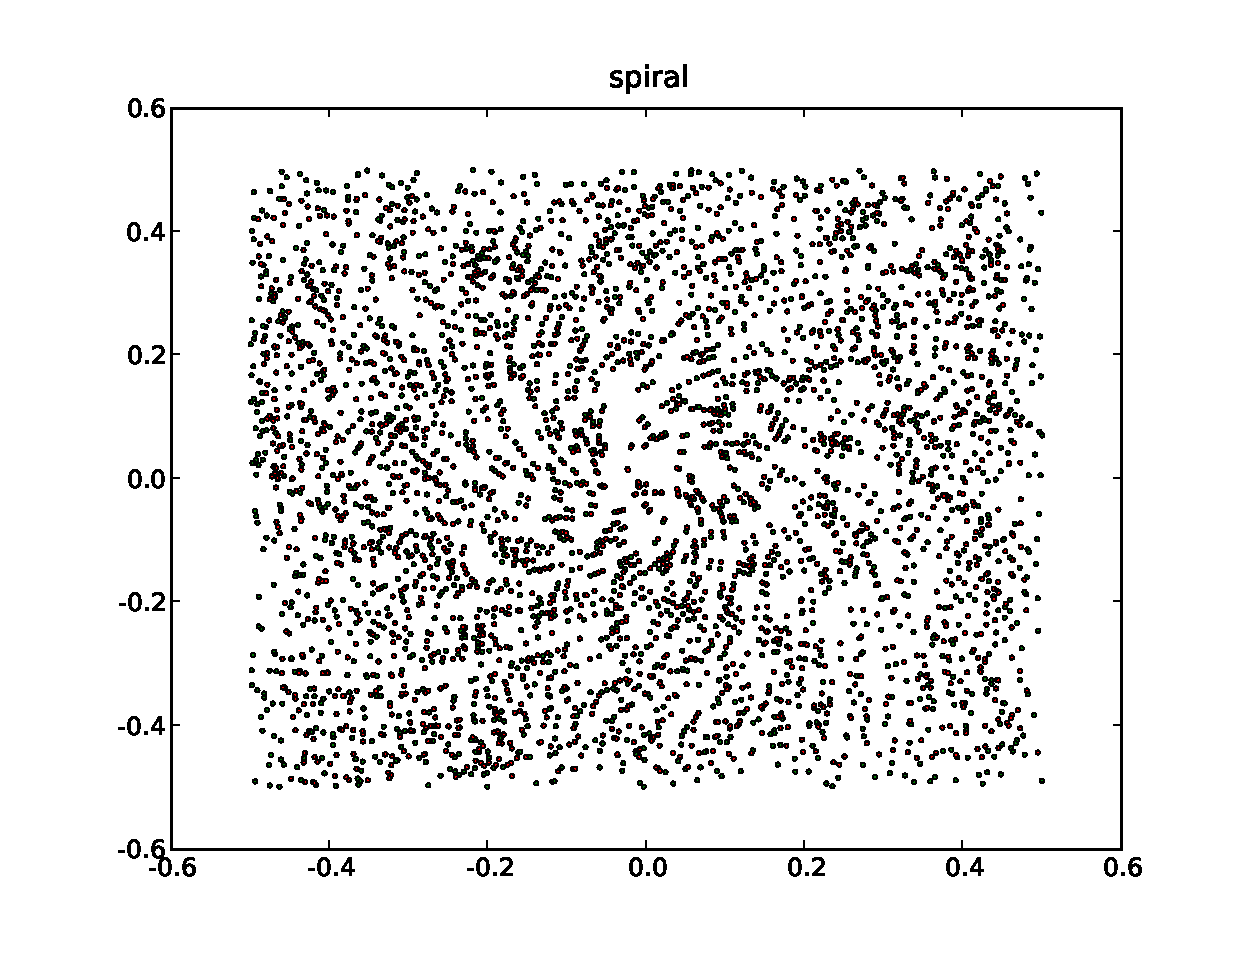
\includegraphics[width=4in]{fig/glass_dots1}\par\end{centering}


\caption{\label{fig:glass_dots1}Glass pattern showing a stable focus}
\end{figure}
\par\end{center}




\end{document}
